\chapter{31 listopada 2015}
\begin{prz}
Niech $ \varepsilon_1,\varepsilon_2,\dots  $ ciąg zmiennych losowych niezależnych o tym samym rozkładzie, skoncentrowanych na $ \mathbb Z $.
\begin{align*}
&X_n=\sum_{j=1}^{n}\varepsilon_j\\
&\forall_{n\neq 1}\;P(\varepsilon_n=k)=\mu_k\qquad
\left(\mu_k\ge 0,\sum_{k=-\infty }^{\infty }\mu_k=1\right)
\end{align*}
$ (X_n)_{n\ge 1} $ jest procesem Markowa o przestrzeni stanów $ S=\mathbb Z $.
\begin{gather*}
P\left(X_{n+1}=j|X_n=i,X_{n-1}=i_{n-1},\dots,X_1=i_1\right)
=\\=
\frac{P\left(X_{n+1}=j,X_n=i,X_{n-1}=i_{n-1},\dots,X_1=i_1\right)}{P\left(X_n=i,X_{n-1}=i_{n-1},\dots,X_1=i_1\right)}
\end{gather*}
\begin{align*}
&\frac{P\left(\varepsilon_{n+1}=j,\varepsilon_n=i,\varepsilon_{n-1}=i_{n-1},\dots,\varepsilon_1=i_1\right)}{P\left(\varepsilon_n=i,\varepsilon_{n-1}=i_{n-1},\dots,\varepsilon_1=i_1\right)}
=\\=&
\frac{P\left(\varepsilon_{n+1}=j\right )P\left (\varepsilon_n=i\right )P\left (\varepsilon_{n-1}=i_{n-1}\right )\dots P\left (\varepsilon_1=i_1\right)}{P\left(\varepsilon_n=i\right )P\left (\varepsilon_{n-1}=i_{n-1}\right )\dots P\left (\varepsilon_1=i_1\right)}
=\\=&
P\left(\varepsilon_{n+1=j-i}\right)=\mu_{j-1}=p_{i,j}
\end{align*}
Mamy własność Markowa. Co więcej jest to łańcuch Markowa jednorodny w czasie $ \left[\mu_{(j+l)+(i+l)}\right] $, ale i jednorodny w przestrzeni.

Jeżeli $ \varepsilon_1,\varepsilon_2,\dots  $ byłyby niezależne, ale o różnych rozkładach, to $ Y_n=X_1+\dots +X_n $ też jest łańcuchem markowa, ale niejednorodnym.
\end{prz}
\begin{twr}[Prawdopodobieństwo ścieżki (path, string, trajektorii)]
Niech $ (X_n)_{n\ge 0} $ będzie łańcuchem Markowa o macierzy prawdopodobieństw przejść $ P=[p_{ij}] $.
\begin{gather*}
P\left(X_{n+k}=i_{n+k},X_{n+k-1}=i_{n+k-1},\dots,X_n=i_n\right)
=\\=
P\left(X_{n+k}=i_{n+k}|X_{n+k-1}=i_{n+k-1},\dots,X_n=i_n\right)
P\left(X_{n+k-1}=i_{n+k-1},\dots,X_n=i_n\right)
\end{gather*}
\end{twr}
\begin{proof}
$ k\ge 0 $ indukcyjnie
\begin{align*}
&p_{i_{n+k-1},i_{n+k}}
p_{i_{n+k-2},i_{n+k-1}}
\dots
p_{i_n,i_{n+1}}
\cdot P\left(X_n=i_n\right)
=\\=&
p_{i_{n=k-1},i_{n+k}}\cdot P\left(X_{n+k-1}=i_{n+k-1},\dots,X_n=i_n\right)
=\\=&
P\left(X_n=i_n\right)\cdot\prod_{\mathclap{l=n+1}}^{\mathclap{{n+k}}}p_{i_{l-1},i_l}
\end{align*}
W szczególności, gdy $ n=0 $
\begin{align*}
&P\left(X_k=i_k,\dots,X_0=i_0\right)
=\\=&
P\left(X_0=i_0\right)\cdot \prod_{l=1}^{k}p_{i_{l-1},i_l}
=\\=&
\mu_{i_0}\cdot\prod_{l=1}^{k}p_{i_{l-1},i_l}
\end{align*}
\end{proof}
Oznaczenie
\begin{gather*}
\mu=\left(\mu_i\right)_{i\in S}=
\mu^{(0)}=
\left(P\left(X_0=i\right)\right)_{i\in S}=
\mathcal L\left(X_0\right)
\end{gather*}
Rozkład początkowy procesu $ \left(X_n\right)_{n\ge 0} $
\begin{align*}
&P\left(X_{n+k}=i_{n+k},\dots,X_{n+1}=i_{n+1}|X_n=i_n,\dots,X_0=i_0\right)
=\\=&
P\left(X_{n+k}=i_{n+k},\dots,X_{n+1}=i_{n+1}|X_n=i_n\right)
\end{align*}
dla dowolnych $ n,k,i,\dots  $.
\begin{proof}
\begin{align*}
&P\left(X_{n+k}=i_{n+k},\dots,X_{n+1}=i_{n+1}|X_n=i_n,\dots,X_0=i_0\right)
=\\=&
\frac{P\left(X_{n+k}=i_{n+k},\dots,X_{n+1}=i_{n+1},X_n=i_n,\dots,X_0=i_0\right)}{P\left(X_n=i_n,\dots,X_0=i_0\right)}
=\\=&
\frac{p_{i_{n+k-1},i_{n+k}}
\dots
p_{i_0,i_1}
\cdot P\left(X_0=i_0\right)}{p_{i_{n-1},i_{n}}
\dots
p_{i_0,i_1}
\cdot P\left(X_0=i_0\right)}
=\\=&
\prod_{l=0}^{n=k-1}p_{i_l,i_{l+1}}
=\\=&
P\left(X_{n+k}=i_{n+k},\dots,X_{n+1}=i_{n+1}|X_n=i_n\right)
\end{align*}
\end{proof}
Własność Markowa (sprzęgająca przeszłość z przyszłością; symetrie przeszłości z przyszłością)\\
$
\mathcal F_{n,\infty}=\sigma\left(X_n,X_{n+1},\dots\right)\\
\mathcal F_{0,n}=\sigma\left(X_0,\dots,X_{n}\right)\\
\mathcal F_{-\infty ,n}=\sigma\left(\dots,X_{n-1},X_n\right)
$
Jeżeli proces stochastyczny $ \left(X_n\right)_{n\ge0} $ spełnia własność Markowa, to
\begin{gather*}
\forall_{\substack{A\in\mathcal F_{0,n}\\B\in \mathcal F_{n,\infty }}}\;
P\left(A\cap B|X_n=i\right)
=
P\left(A|X_n=i\right)P\left(B|X_n=i\right)
\end{gather*}
Warunek Markowa $ \equiv  \mathcal F_{0,n}$ i $ \mathcal F_{n,\infty } $ są warunkowo $ X_n $ niezależne.

Równość wystarczy udowodnić dla 
\begin{align*}
&A=\left\{X_0=i_0,\dots,X_{n-1}=i_{n-1},X_n=i\right\}\\
&B=\left\{X_n=i,X_{n+1}=i_{n+1},\dots,X_{n+k}=i_{n+k}\right\}\in C_{n,n+k}
\end{align*}
\begin{proof}
\begin{align*}
&P\left(A\cap B|X_n=i\right)
=\\=&
\frac{P\left(A\cap B\cap\{X_n=i\}\right)}{P\left(X_n=i\right)}
=\\=&
\frac{P\left(X_{n+k}=i_{n+k},\dots,X_{n+1}=i_{n+1},X_n=i,X_{n-1}=i_{n-1},\dots,X_0=i_0\right)}{P\left(X_n=i,\dots,X_0=i_0\right)}
\cdot\\\cdot&
\frac{P\left(X_n=i,\dots,X_0=i_0\right)}{P\left(X_n=i\right)}
=\\=&
P\left(X_{n+k}=i_{n+k},\dots,X_{n+1}=i_{n+1},X_n=i|X_n=i,\dots,X_0=i_0\right)
\cdot\\\cdot&
P\left(X_n=i,\dots,X_0=i_0|X_n=i\right)
=\\=&
P\left(A|X_n=i\right)
P\left(B|X_n=i\right)
\end{align*}
\end{proof}
\section{Mocna własność Markowa}
\begin{twr}[Mocna własność Markowa]
Niech $ \left(X_n\right)_{n\ge0 } $ będzie łańcuchem Markowa, jednorodnym o macierzy prawdopodobieństw przejść $ P=\left[p_{ij}\right] $. Jeżeli $ T $ jest momentem Markowa względem filtracji naturalnej) to proces stochastyczny
\begin{gather*}
Y_n\stackrel{df}{=}X_{n+T}\qquad,n=0,1,\dots 
\end{gather*}
jest też łańcuchem Markowa o macierzy prawdopodobieństw przejść $ \left[p_{ij}\right] $.
\begin{proof}
\begin{align*}
&P\left(Y_{n+1}=j|Y_n=i,Y_{n-1}=i_{n-1},\dots,Y_0=i_0\right)
=\\=&
P\left(X_{n+1+T}=j|X_{n+T}=i,X_{n-1+T}=i_{n-1},\dots,X_T=i_0\right)
=\\=&
\frac{P\left(X_{n+1+T}=j,X_{n+T}=i,X_{n-1+T}=i_{n-1},\dots,X_T=i_0\right)}{P\left(X_{n+T}=i,X_{n-1+T}=i_{n-1},\dots,X_T=i_0\right)}
=\\=&
\frac{\sum_{k=0}^{\infty }P\left(X_{n+1+T}=j,X_{n+T}=i,X_{n-1+T}=i_{n-1},\dots,X_T=i_0,T=k\right)}{\sum_{k=0}^{\infty }P\left(X_{n+T}=i,X_{n-1+T}=i_{n-1},\dots,X_T=i_0,T=k\right)}
=\\=&
\frac{\sum_{k=0}^{\infty }P\left(X_{n+1+k}=j,X_{n+k}=i,X_{n-1+k}=i_{n-1},\dots,X_k=i_0,T=k\right)}{\sum_{k=0}^{\infty }P\left(X_{n+k}=i,X_{n-1+k}=i_{n-1},\dots,X_k=i_0,T=k\right)}=
\end{align*}
Zauważmy, że zachodzi
\begin{gather*}
\left\{T=k\right\}\in\sigma\left\{X_0,X_1,\dots,X_k\right\}\\
\left\{T=k\right\}=\dot {\bigcup_m}\underbrace{\left\{X_k=m_k,\dots,X_0=m_0\right\}}_{\text{atom}}
\end{gather*}
wykorzystując powyższy opis
\begin{align*}
&\frac{\sum_{k=0}^{\infty }P\left(X_{n+1+k}=j,X_{n+k}=i,X_{n-1+k}=i_{n-1},\dots,X_k=i_0,\dot {\bigcup\limits_m}\left\{X_k=m_k,\dots,X_0=m_0\right\}\right)}
{\sum_{k=0}^{\infty }P\left(X_{n+k}=i,X_{n-1+k}=i_{n-1},\dots,X_k=i_0,\dot {\bigcup\limits_m}\left\{X_k=m_k,\dots,X_0=m_0\right\}\right)}
=\\=&
\frac{\sum_{k=0}^{\infty }\sum_mP\left(X_{n+1+k}=j,X_{n+k}=i,X_{n-1+k}=i_{n-1},\dots,X_k=i_0,X_k=m_k,\dots,X_0=m_0\right)}
{\sum_{k=0}^{\infty }\sum_mP\left(X_{n+k}=i,X_{n-1+k}=i_{n-1},\dots,X_k=i_0,X_k=m_k,\dots,X_0=m_0\right)}
=\\=&
\frac{\sum_{k=0}^{\infty }\sum_mP\left(X_{n+1+k}=j|X_{n+k}=i,X_{n-1+k}=i_{n-1},\dots,X_k=i_0,X_k=m_k,\dots,X_0=m_0\right)}
{\sum_{k=0}^{\infty }\sum_mP\left(X_{n+k}=i,X_{n-1+k}=i_{n-1},\dots,X_k=i_0,X_k=m_k,\dots,X_0=m_0\right)}\\&
\frac{P\left(X_{n+k}=i,X_{n-1+k}=i_{n-1},\dots,X_k=i_0,X_k=m_k,\dots,X_0=m_0\right)}{}
=\\=&
\frac{\sum_{k=0}^{\infty }\sum_mp_{ij}P\left(X_{n+k}=i,X_{n-1+k}=i_{n-1},\dots,X_k=i_0,X_k=m_k,\dots,X_0=m_0\right)}
{\sum_{k=0}^{\infty }\sum_mP\left(X_{n+k}=i,X_{n-1+k}=i_{n-1},\dots,X_k=i_0,X_k=m_k,\dots,X_0=m_0\right)}
=\\=&
p_{ij}\frac{\sum_{k=0}^{\infty }\sum_mP\left(X_{n+k}=i,X_{n-1+k}=i_{n-1},\dots,X_k=i_0,X_k=m_k,\dots,X_0=m_0\right)}
{\sum_{k=0}^{\infty }\sum_mP\left(X_{n+k}=i,X_{n-1+k}=i_{n-1},\dots,X_k=i_0,X_k=m_k,\dots,X_0=m_0\right)}
=\\=&
p_{ij}
\end{align*}
\end{proof}
\end{twr}
Rozkład początkowy $ Y_0 $?
\begin{gather*}
P\left(Y_0=i\right)=P\left(X_T=i\right)=\sum_{k=0}^{\infty }P\left(X_k=i,T=k\right)
\end{gather*}
\textbf{Wniosek}\\
\begin{gather*}
P\left(X_{T+n}=j|X_T\right)=p_{X_T,j}^{(n)}\\
\mathbb E \left(\mathbbm1_{\left\{X_{T+n}=j\right\}}|X_T\right)=p_{X_T,j}^{(n)}
\end{gather*}
Grafowa wizualizacja łańcucha Markowa\\
Stany - wierzchołki grafu\\
Prawdopodobieństwa przejść $ [p_{ij}] $ - krawędzie skierowane tylko te, gdzie $ p_{ij}>0 $
\begin{center}
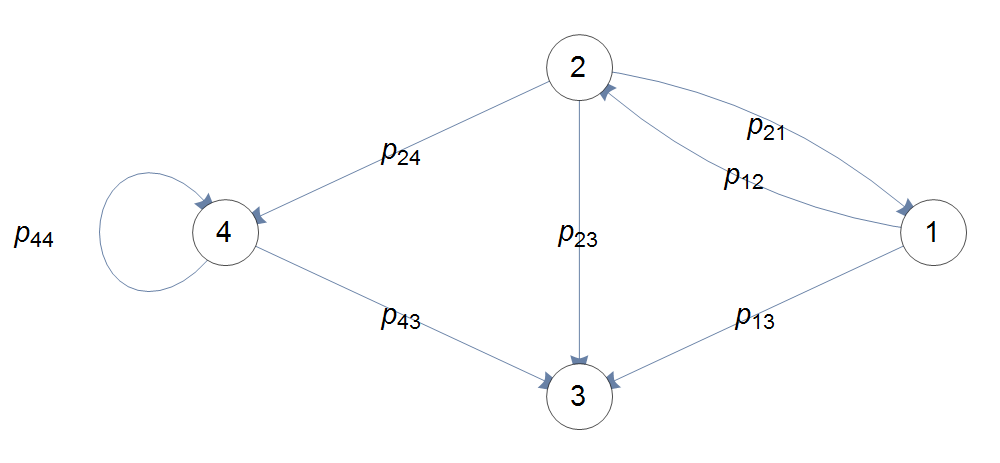
\includegraphics[width=0.7\linewidth]{graf}
\end{center}
\begin{defi}
Niech $ \left(X_n\right)_{n\ge0} $ będzie łańcuchem Markowa. Mówimy, że stan $ j\in S $ jest osiągalny ze stanu $ i\in S $, jeżeli istnieje $ n\ge0 $, że $ P\left(X_n=j|X_0=i\right)>0 $.
\end{defi}
\begin{itemize}
\item $ p_{i,j}^{(n)}>0 $
\item $ p_{i,j}^{[0,n]}>0 $
\end{itemize}
$ p_{i,j}^{[0,n]}>0 $ dla niejednorodnego łańcucha markowa nie Będzie przedmiotem rozważań.\\
Piszemy wtedy $ i\longrightarrow j $ dokładniej $ i\xrightarrow{\text{"n"}}j $
\begin{gather*}
\equiv P\left(X_0=i,X_1=i_1,\dots,X_{n-1}=i_{n-1},X_n=j\right)>0
\end{gather*}
dla pewnej ścieżki $ \left[i,i_1,i_2,\dots,i_{n-1},j\right] $
\begin{defi}
Mówimy, że stan $ i,j<in S $ komunikują się, gdy $ i\longrightarrow j $ oraz $ j\longrightarrow i $
\begin{gather*}
\left[
p_{ij}^{(n)}>0\wedge
p_{ji}^{(m)}>0
\right]
\end{gather*}
Piszemy wtedy
\begin{gather*}
i\longleftrightarrow j
\end{gather*}
\end{defi}
\begin{twr}
Relacja komunikowania się $ \longleftrightarrow $ jest relacją równoważności.
\begin{proof}
\begin{enumerate}
\item Zwrotność $ i\longleftrightarrow i $
\begin{gather*}
p_{ii}^{(0)}=1>0
\end{gather*}
\item Symetria $ i\longleftrightarrow j\stackrel{df}{\Leftrightarrow}i\longrightarrow j\wedge j\longrightarrow i $
\item Przechodniość $ i\longleftrightarrow j \wedge j\longleftrightarrow k\Rightarrow i\longleftrightarrow k$\\
$ i\longleftrightarrow k $?\\
$ i\longrightarrow j\wedge j\longrightarrow k $\\
$ p_{ij}^{(n)}>0 \wedge p_{jk}^{(m)}>0 $
\begin{gather*}
p_{ik}^{(n=k)}\stackrel{GK}{=}\sum_{l\in S}p_{il}^{(n)}p_{lk}^{(m)}\ge p_{ij}^{(n)}p_{jk}^{(m)}
\end{gather*}
Zatem $ i\longrightarrow k $. Analogicznie $ k\longrightarrow i $.
\end{enumerate}
\end{proof}
\end{twr}
\textbf{Wniosek.}\\
przestrzeń stanów $ S=\dot \bigcup[i]_{/\leftrightarrow},\,[i]_{/\leftrightarrow}= \left\{j\in S:i\longleftrightarrow j\right\}$
\begin{gather*}
S_{/\leftrightarrow}\quad \text{przestrzeń ilorazowa}
\end{gather*}
Przestrzeń stanów dzieli się na rozłączne klasy. Niektóre klasy są jednoelementowe. Czasami $ [i]_{\leftrightarrow}=\left\{i\right\} $
\begin{defi}
Dla ustalonego łańcucha Markowa $ \left(X_n\right)_{n\ge 0} $ o macierzy prawdopodobieństw przejść $ P=\left[p_{ij}\right] $ okresem stanu $ i $ nazywamy liczbę
\begin{gather*}
d(i)=NWD\left\{n\ge0:p_{ij}^{(n)}>0\right\}=
NWD\left\{n-m:pp_{ij}^{(n)},P_{ij}^{(m)}>0\right\}
\end{gather*}
\end{defi}
\textbf{Uwaga!}\\
Jeżeli $ \forall_{n\ge 1}\;p_{ii}^{(n)}=0 $, to $ d(i)=\infty  $.\\
Jeżeli $ d(i)=1 $, to stan $ i $ nazywamy aperiodycznym.
\begin{prz}
\begin{gather*}
P\left(X_{n+1}=j|X_n=i\right)=\left \{
\begin{array}{lll}
	p & j=i+1            &  \\
	q & j=i-1            &  \\
	0 & \text{pozostałe} &
\end{array}
\right .
\end{gather*}
$ P_{ii}^{(2n)}>0\\
p_{ii}^{(2n+1)}\equiv0 $\\
Konkluzja
\begin{gather*}
\forall_{i\in \mathbb Z}\;d(i)=d=2.
\end{gather*}
$ i\longleftrightarrow j $ dla dowolnych $ i,j\in \mathbb Z $
\end{prz}
\begin{defi}
Niech $ \left(X_n\right)_{n\ge 0} $ będzie jednorodnym łańcuchem Markowa. Mówimy, że łańcuch Markowa jest nieprzewiedlny (\emph{irreducible}), jeśli
\begin{gather*}
\forall_{i,j\in S}\;i\longleftrightarrow j.
\end{gather*}
\end{defi}